\documentclass[addpoints, 11pt]{exam}
\usepackage{url}
\usepackage{amsmath,amsthm,enumitem}
\usepackage{graphicx}
%\input myfonts

\newtheorem*{claim}{Claim}
\title{CS 6150: HW3 -- Greedy algorithms, Graphs basics}
\date{Submission date: Monday, Oct 25, 2021 (11:59 PM)}
\begin{document}
\maketitle
\begin{center}
\fbox{\fbox{\parbox{5.5in}{\centering
This assignment has \numquestions\ questions, for a total of \numpoints\
points. % and \numbonuspoints\ bonus points.  
Unless otherwise specified, complete and reasoned arguments will be expected for all answers. }}}
\end{center}

\qformat{Question \thequestion: \thequestiontitle\dotfill \textbf{[\totalpoints]}}
\pointname{}
\bonuspointname{}
\pointformat{[\bfseries\thepoints]}

\begin{center}
  \gradetable
\end{center}
\newpage
\paragraph{Instructions.}  For all problems in which you are asked to develop an algorithm, write down the pseudocode, along with a rough argument for correctness and an analysis of the running time (unless specified otherwise). Failure to do this may result in a penalty. If you are unsure how much detail to provide, please contact the instructors on Piazza.

\begin{questions}
\titledquestion{Set Cover Analysis}
In class, we saw the set cover problem (phrased as picking the smallest set of people who cover a given set of skills). Formally, we have $n$ people, and each person has a subset of $m$ skills. Let the set of skill set of the $i$th person be denoted by $S_i$, which is a subset of $[m]$ (shorthand for $\{1, 2, \dots, m\}$). We analyzed a greedy algorithm that at every step, selects the person with the largest number of {\em uncovered} skills.
\begin{parts}
\part[2] First, let us show that our analysis cannot be improved significantly. Consider the instance given by Figure~\ref{fig:set-cover} (with $n=5$ people and $m=26$), and write down (i) the optimal solution, and (ii) the solution output by the greedy algorithm.

\begin{figure}[!h]
\begin{center}
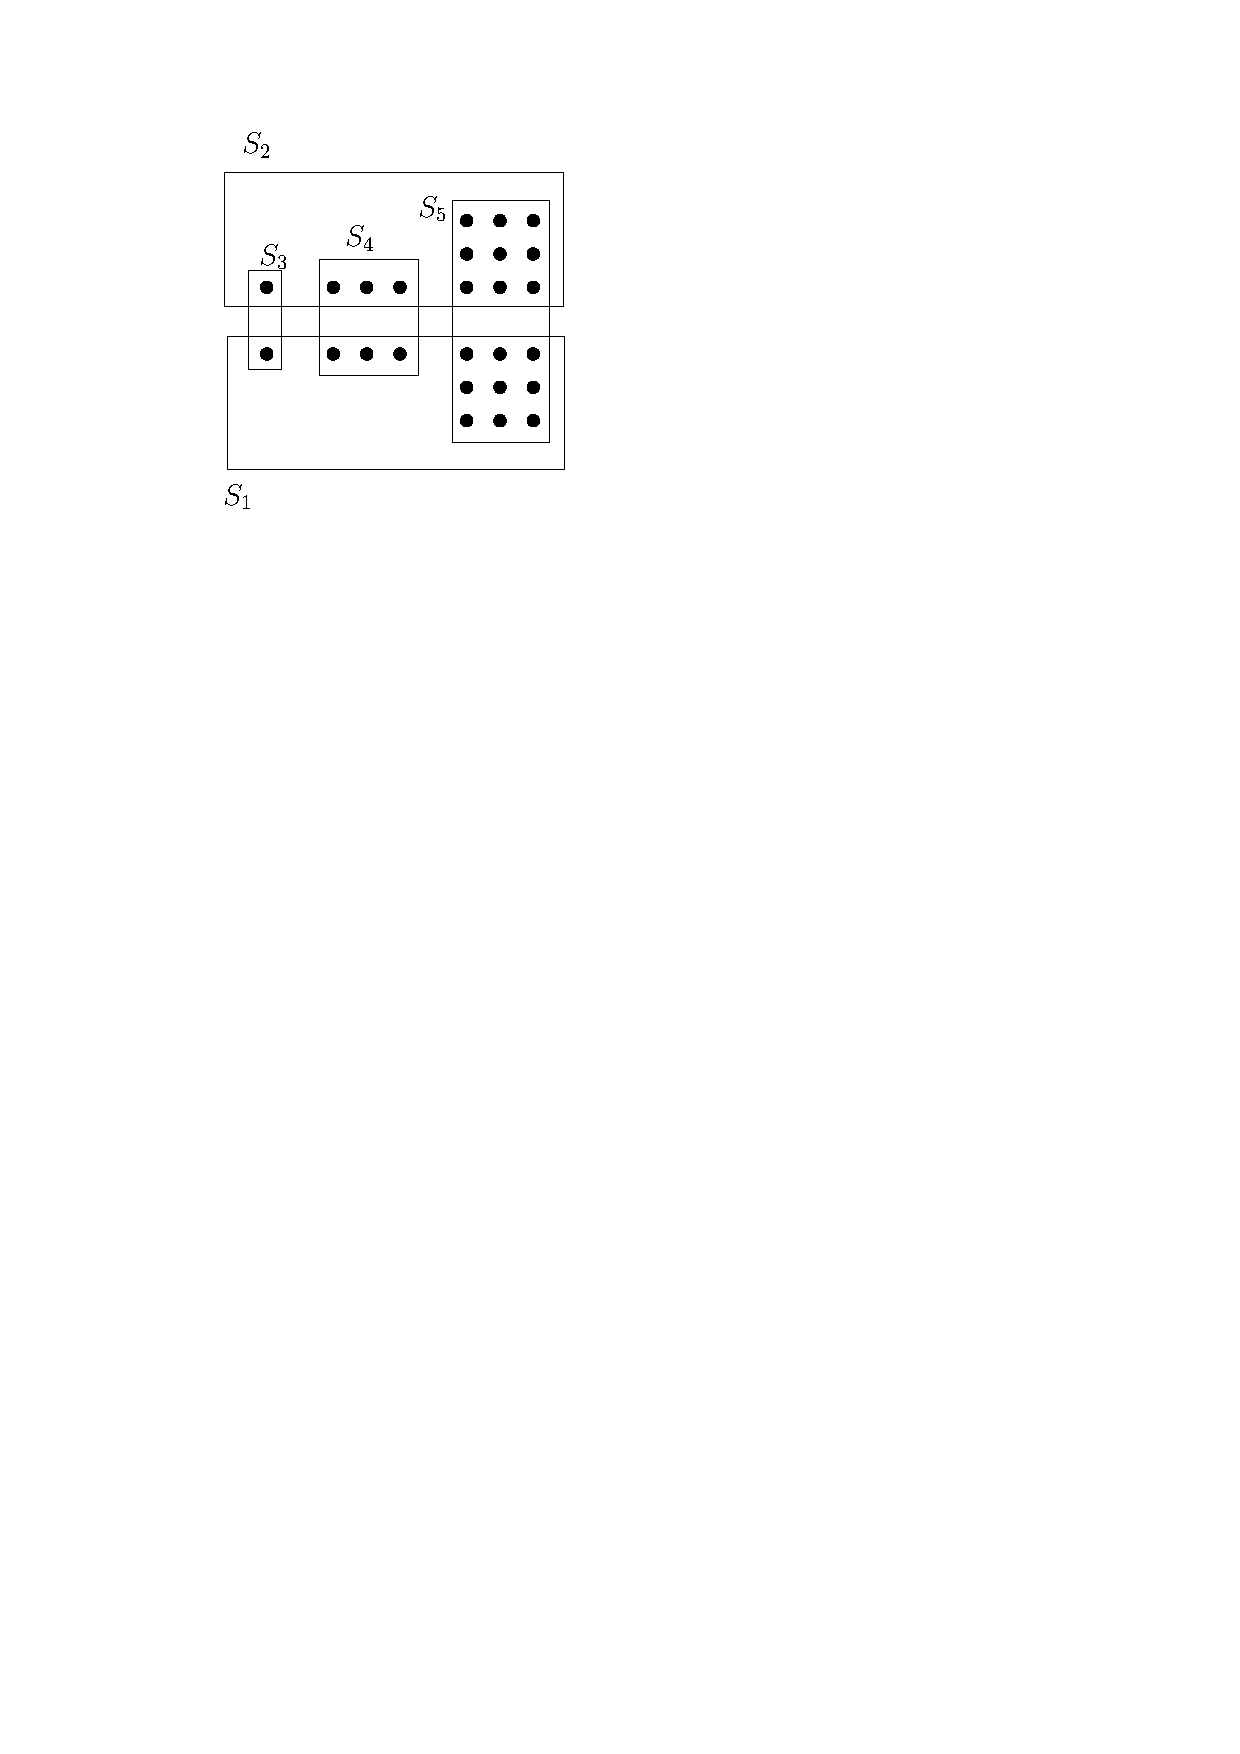
\includegraphics[scale=0.7]{hw3-fig1.pdf}
\caption{Every dot represents a skill, the rectangles show the skill sets of the people 1, 2, ..., 5.}
\label{fig:set-cover}
\end{center}
\end{figure}

\part[6] Using Figure~\ref{fig:set-cover} as a hint, describe an instance in which the ratio of the size of the solution produced by the greedy algorithm and the size of the optimal solution is $\Omega(\log m)$. 
 
\part[6] Next, let us see what happens if we stop the algorithm ``mid way''. Suppose we are given a parameter $k$, and we are told that there is a set of $k$ people whose skill sets cover all of $[m]$. Now, suppose we run the greedy algorithm for exactly $k$ iterations. So the algorithm chooses exactly $k$ people, but it could be that some of the skills are still uncovered. Prove, however, that at least $50\%$ of the skills are covered.  [{\em Hint:} Modify the proof we saw in class.]
\end{parts}

\titledquestion{Be lazy or be greedy?}
Consider the following ``street surveillance'' problem. We have a graph $(V, E)$ with $|V| = n$ nodes and $|E| = m$ edges. We are allowed to place surveillance cameras at the nodes. Once placed, they can monitor all the edges incident to the node. The goal is to place as few cameras as possible, so as to monitor {\bf all the edges} in the graph.
\begin{parts}
\part[4] Show how to ``cast'' the street surveillance problem as an instance of Set Cover, and write down the greedy algorithm. (You don't need to provide any analysis.)
\part[7] Let $(V, E)$ be a graph as above, and now consider the following ``lazy'' algorithm: 
\begin{enumerate}
\item initialize $S = \emptyset$
\item while there is an unmonitored edge $\{i,j\}$:  \\
		$~~~~~~$add both $i, j$ to $S$ and mark all their edges as monitored
\end{enumerate}
Clearly (due to the while loop), the algorithm returns a set $S$ that monitors all the edges.  Prove that this set satisfies $|S| \le 2k$, where $k$ is the size of the optimal solution (i.e., the minimum number of nodes we need to place cameras at in order to monitor all the edges).

{\sc Moral.}  Even though the algorithm looks ``dumber'' than the greedy algorithm, it has a better approximation guarantee --- $2$ versus $\log n$.
\end{parts}

{\em Hint.} Consider the edges $\{i,j\}$ encountered when we run the algorithm. Could it be that the optimal set chooses {\em neither} of $\{i,j\}$?

\titledquestion{Finding triangles}
We will now see how for some graph problems, ``non-standard'' approaches can sometimes yield efficient algorithms. Let $(V, E)$ be the set of vertices and edges in a directed graph, respectively. 

Our goal is to find out if the graph has a {\em triangle}, i.e., if there exist $i,j, k \in V$ such that $(i,j), (j,k)$ and $(k,i)$ all belong to $E$. 
\begin{parts}
\part[3] Show how to do this in time $O\left( \sum_{i \in V} d_{in}(i) d_{out} (i) \right)$, where $d_{in}$ and $d_{out}$ refer to the in-degree and out-degree of a vertex respectively.
\part[6] Of course, the above reduces to $O(n^3)$ if the graph is dense and $d_{in}$ and $d_{out}$ are $\Theta(n)$ for many vertices. However, assuming that two $n \times n$ matrices can be multiplied in time $O(n^{2.4})$ (which is known to be true), show how to solve the problem in time $O(n^{2.4})$.  [{\em Hint:}  Consider the adjacency matrix of the graph $A$.  What can you say about the entries of $A \cdot A$? Can you use this matrix to then check the existence of a triangle?]
\end{parts}

\newcommand{\opt}{\textsc{Opt}}
\titledquestion{Road tripping}
Let us roll back to the days when a road trip meant writing all your favorite music onto CDs and carrying them along.

Suppose we have $n$ songs, of durations $d_1, d_2, \dots, d_n$, where each $d_i$ is less than one hour. Suppose that every CD can hold one hour of music. The goal is to write all the songs to a set of CDs, so as to minimize the number of CDs required.

Consider the natural greedy algorithm for the problem: at every step, we have a list of CDs containing the music written so far (initially empty). Now consider the songs in the given order, and for song $i$, write it to the \underline{first CD so far} that has sufficient space for the song. If there is no such CD, then we buy a new CD, and write song $i$ to it (and add it to the CD list; we are assuming that we can keep adding songs to a CD as long as there is space).

\begin{parts}
\part[3] Give an example in which the greedy algorithm is not optimal. I.e., give a set of song durations for which the above procedure uses more CDs than an optimal ``packing''.
\part[7] Suppose you are told that all the song durations are at most 20 minutes. Now prove that the greedy algorithm is  within a factor $3/2$ of the ``best possible'' number of CDs. In other words, prove that if $\opt$ denotes the number of CDs in the best-possible solution, then the algorithm uses $\le (1.5 \cdot \opt)$ CDs. You will get full credit even if your bound is off by an additive constant, e.g., you prove $\le (1.5 \cdot \opt + 2)$. [{\em Hint:} You may want to compare the number of CDs used by the algorithm with the ``total duration'' of the songs.  Also, play around with small examples to see how the algorithm is doing.]
\end{parts}

\titledquestion{Santa's tradeoffs}[6]
Recall the matching problem we saw in class: there are $n$ gifts, and $n$ children, and each child has a non-negative valuation for each gift. Formally, the value of gift $j$ to child $i$ is given by $H_{i,j}$.  We assume that all $H_{i,j} \ge 0$. Santa's goal is to give one gift to each child, so as to maximize the {\em total value} (of course, a gift cannot be given to more than one child).

Suppose we now perform a more elaborate local search, this time picking every {\em triple} of edges in the current solution, and seeing if there is a reassignment of gifts between the end points of these edges that can improve the total value. Prove that a locally optimal solution produced this way has a value that is at least $(2/3)$ the optimum value. [This kind of a trade-off is typical in local search -- each iteration is now more expensive $O(n^3)$ instead of $O(n^2)$, but the approximation ratio is better.]

{\bf Note.}  We will see in the coming lectures that this problem can indeed be solved optimally in polynomial time, using a rather different algorithm. 

\end{questions}
\end{document}